\scanpage{120}

\diagram{\tikz[baseline=(a.base)]\node[draw,ellipse,inner sep=2pt](a){$i\geq n$};\quad
$\boxed{\begin{array}{l|c|c|c|c|c|c|c|c|c}
\text{poids}&2(i-n)+2&2(i-n)+3&2(i-n+4)&\raisebox{-.6ex}{$\times$}&i&i+1&i+2&\cdots&2n\\\hline
\text{niveau}&0&1&2&&\substack{2n-i\\-2}&2n-i-1&2n-i-2&\text{---}&0
\end{array}}$}

\figure{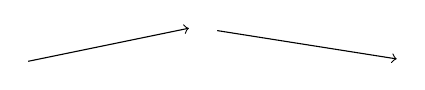
\begin{tikzpicture}[x=.6cm,y=.6cm]\draw[->] (0,0)--(3.4,.7);\draw[->] (4,.65)--(7.8,.05);\end{tikzpicture}}

\[
\begin{aligned}
&\text{poids }\underline{2n}\ \text{intervient avec }\deleted{\unsure{R^{2n}}},\quad
E_2^{2(i-n),2n-i}=\sum R^{2(i-n)}f_{\underbrace{Z_{\alpha_1}\cap Z_{\alpha_2}\cdots\cap Z_{\alpha_{2n-i}}}_{\dim\,i-n}}(\mathbb Q_\ell)(-2n+i)\\
&\qquad 2n-i\leq n\leq i\qquad\qquad n-(2n-i)=i-n\\
&\hspace{9em}2(i-n)+2(2n-i)=2n
\end{aligned}
\]

\diagram{$\boxed{\begin{array}{l|c|c|c|c|c|c|c|c|cc}
i&0&1&\cdots&n-1&\unsure{n|-}&n+1&\cdots&2n-1&\deleted{\leq 2n}&\leq 2n-1\\\hline
\text{niveau}&0&1&\cdots&n-1&n-1&n-2&\cdots&0&&\leq n-1\\\hline
\text{poids }\leq&0&2&&2n-2&2n,&2n&2n&2n&&\leq 2n
\end{array}}$}

\[ \boxed{\begin{aligned}\text{poids}&\leq 2\operatorname{Inf}(\deleted{\unsure{2}}i,\deleted{\unsure{2}}n)\\
\text{niveau}&\leq\operatorname{Inf}(i,n-1)\end{aligned}} \]

Si $F$, \deleted{\unsure{str|str$^{\rm t}$}} spécial de poids $i$

\[ \begin{aligned}\text{poids}&\leq 2\operatorname{Inf}(i,n)+j\quad ?\\
\text{niveau}&\leq\operatorname{Inf}(i,n-1)+j\end{aligned} \]

\deleted{\textcircled{\unsure{2|2\textsuperscript{o}}} $f$ \unsure{séparé de t.f.}, $F=\mathbb Q_{\ell X}$}

% slanted
\margin{Cas général relatif en \unsure{gardant} \unsure{même} $n$}

\diagram{\begin{tikzcd}[ampersand replacement=\&] X\arrow[d,"f"]\\Y\ni y \end{tikzcd}}

\[ n\deleted{\unsure{d_y|=y}}=d_y(f)=\underset{\substack{x\in X\\\text{t.q. }f(x)\in\operatorname{Sp}\mathcal O_{Y,y}}}{\operatorname{Sup}}
\left[\deg \mathrm{tr}\,[k(x):k(f(x))]+{}\deleted{\unsure{d|{+}}}\dim\left(\overline{f(x)}\big/ \unsure{y\ d_y|y}\right)\right. \]

\margin{au vois. de \deleted{\unsure{$x$}} $y$}

\[ \boxed{\begin{aligned}\text{poids}&\leq 2\operatorname{Inf}(i,n)+j\\
\text{niveau}&\leq\operatorname{Inf}(i,n)+j\end{aligned}}\quad ? \]

\margin{peut se remplacer par $n-1$ si $f$ est \deleted{à fibres \unsure{non}} \unsure{de dim|ou dim} $\leq n-1$ ?}

% archive sheet number: 119
